
\newcommand{\credIdentifier}{\footnote{There is a requirement to check whether the credential identifier, generated by the Authenticator
device exsits on the server.
For further discussions on this topic, see section \hyperref[sec:futurework]{Future work}}}

\newcommand{\navigatorApi}{\footnote{In LessPM's case, this is the \textit{navigator.credentials} API provided by the browser.}}


WebAuthn, short for Web Authentication, is a collaborative project between the FIDO Alliance and W3C that aims to
implement a secure, robust key-based authentication system for the web, to strongly authenticate users~\cite{webauthn_level_2}.
The concept relies on the use of a third-party device, called an Authenticator, which leverages asymmetric cryptography.
These devices employ biometric or hardware-based mechanisms to provide a secure and reliable means of authenticating a
user.

Upon registration, the Authenticator device generates a key pair called a Passkey.
This Passkey contains a credential ID uniquely generated for each registered key-pair~\cite{webauthn_credential_id,webauthn_public_key_credential}
on the Authenticator.
The unique generation of each key pair offers the advantage of making it much more difficult for trackers to follow a user
\footnote{This is subject to the key-pair alone. A willing party could still track the user through their email or similar.}.
Further, if an attacker gains access to an individual's Passkey, they might compromise one specific service, whereas
a traditional password could potentially compromise multiple services where password reuse occurs\cite{wang2018next}.

\subsubsection{Registration}\label{subsubsec:registration}
In order to register in a WebAuthn authentication system, the user (i.e., client, browser, phone, etc.) issues a registration request to a
WebAuthn implemented server, called a Relying Party (RP), asking to be registered.
The request contains a body with the relevant user identifier (UID. i.e., username, phone number, email, etc.).
The server responds by initiating a Registration Ceremony (RC) and generates a challenge, which is sent to the client.

The client then calls the browser-integrated WebAuthn API, requesting the Authenticator (i.e., phone, hardware authenticator device, or similar)
to create a new public key credential.\footnote{
  The user is prompted to use their Authenticator to prove their presence, which can involve scanning a QR code,
  providing a fingerprint, or any other modality supported by the device.}
During this process, the Authenticator generates a new key-pair (public and private keys). The Authenticator then signs the challenge received from the server with the private key.

The newly created public key, signed challenge, and additional metadata are combined into a public key credential object,
which the client sends back to the server.

The server verifies the authenticity of the signed challenge and the public key credential object.
If successful, the server stores the user's public key and other relevant information (e.g., user identifier, credential ID)
for future authentication.
Thus completing the RC\@.

The process can be seen in~\ref{fig:registration}.
\begin{figure}[htbp]
  \centering
  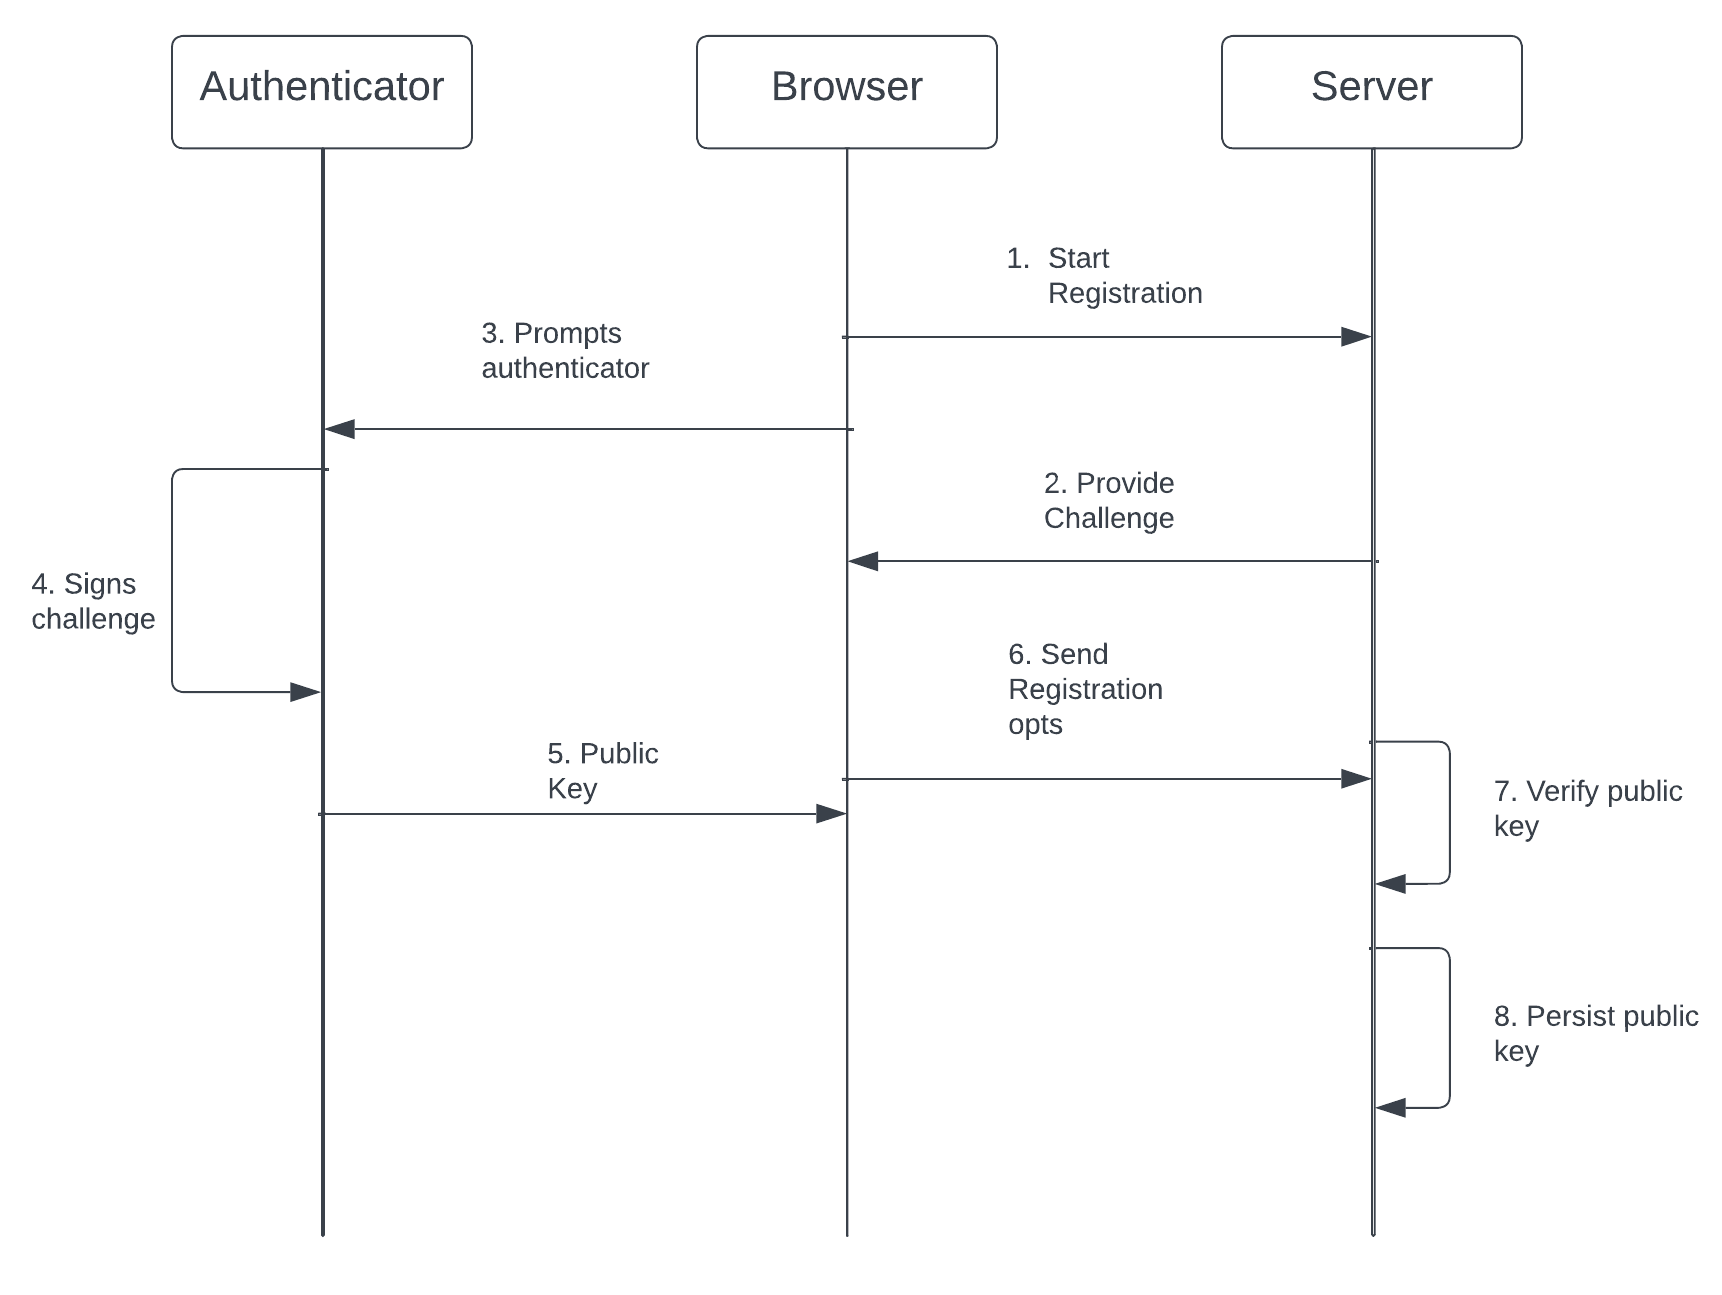
\includegraphics[width=0.75\linewidth]{images/Registration}
  \caption{\footnotesize A diagram dipicting the registration process through WebAuthn and Authenticator Device.}
  \label{fig:registration}
\end{figure}

\subsubsection{Authentication}\label{subsubsec:authentication}
When a user wishes to perform authentication (commonly referred to as \texttt{logging in}), much of the same procedure
occurs.
The user issues an authentication request to the RP, asking for authentication
with the UID that the user used to sign up included in the request body.
If the server can find an associated user with the UID in the persisted storage,
the server responds by initiating and issuing an Authentication Ceremony (AC)
containing a challenge.

The client calls the browser-integrated WebAuthn API, prompting the use of the
Authenticator to validate and sign the challenge.
Unlike the registration process, the Authenticator now yields a signature, which is forwarded to the RP along with
Authenticator-specific data~\cite{webauthn_authenticator_data}.
Upon receiving the data, the Relying Party (RP) validates the signed challenge using the stored credentials.
If the validation succeeds, the server authenticates the user.

The RP can then determine the next steps, such as deciding the authentication
duration and establishing methods for persisting and validating the
authentication.\footnote{
  In the case of LessPM, the system sets an authentication duration of 15 minutes.
  It stores this information within an AES256 encrypted~\ref{subsec:aes} JSON
  Web Token.
  For more details about this process, refer to Section~\ref{subsec:jsonwebtokens}.
} If the authentication process is unsuccessful at any point in the ceremony,
the ceremony is aborted and considered invalid.


This process can be seen in Figure~\ref{fig:authentication}.

\begin{figure}[htbp]
  \centering
  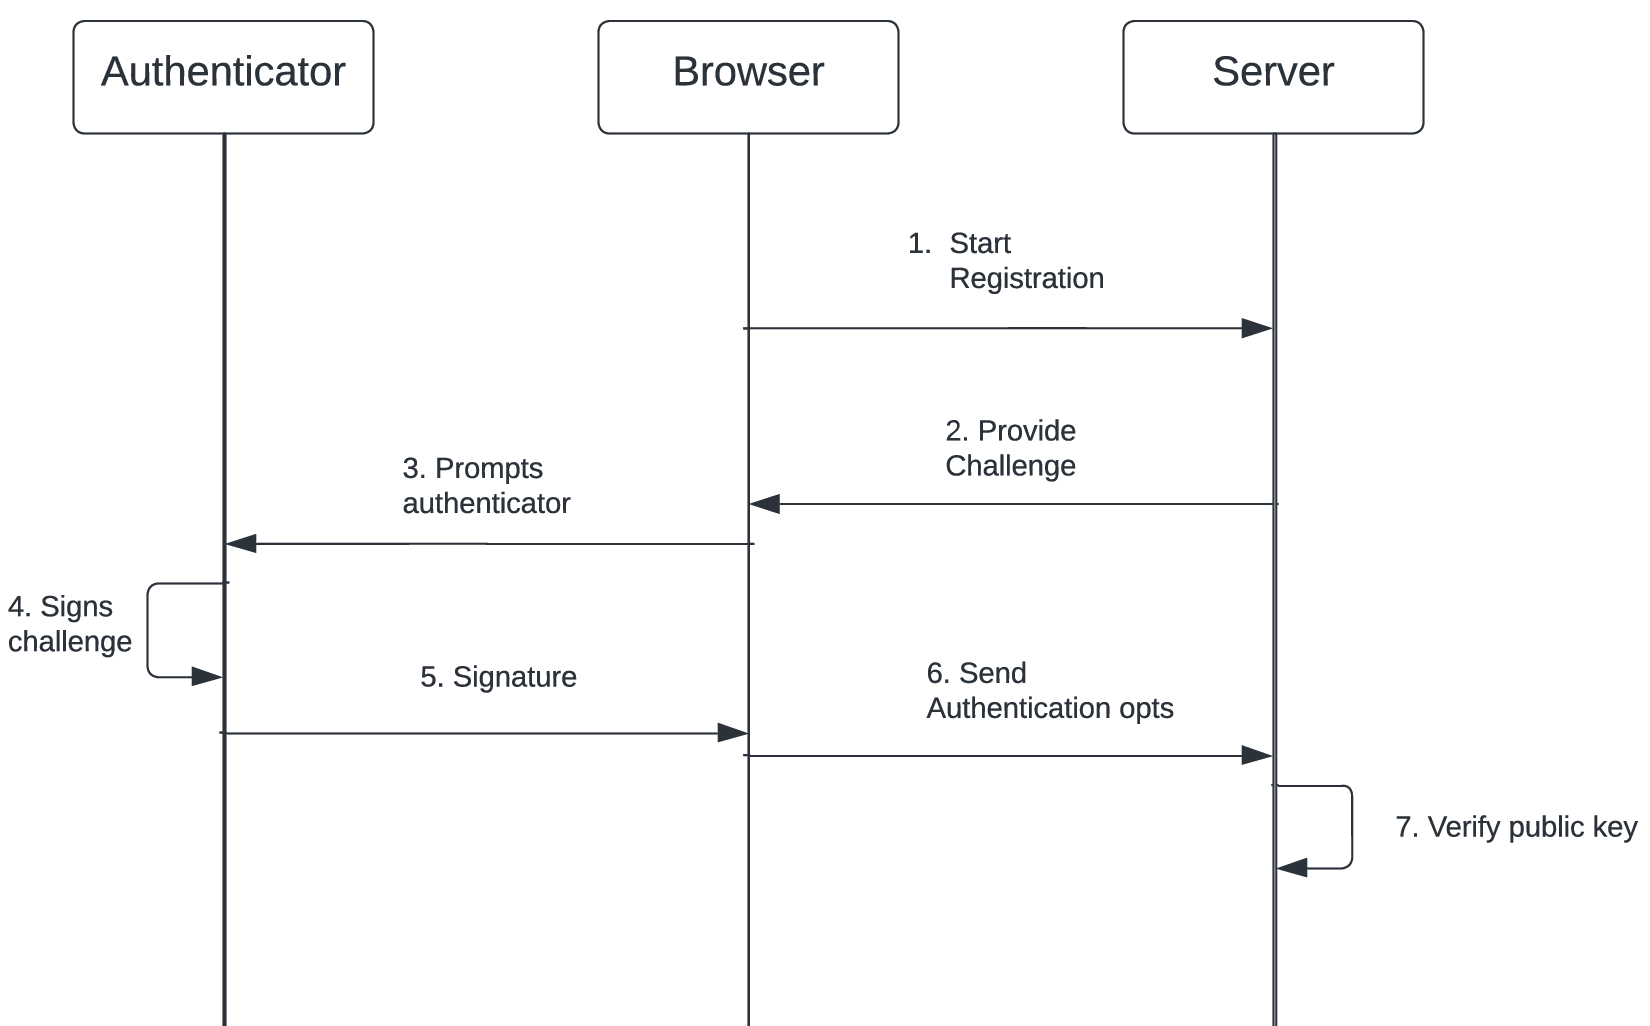
\includegraphics[width=0.8\linewidth]{images/Authentication}
  \caption{\footnotesize A diagram dipicting the authentication process through WebAuthn and Authenticator Device.}
  \label{fig:authentication}
\end{figure}